\chapter{Introdução}
\label{cap:introducao}
A Web é baseada em documentos, onde os documentos ou páginas são descritas através de uma linguagem de marcação de hipertexto (HTML) e interligados através de \textit{hiperlinks}. Para acessar as páginas na Web, é necessário um mecanismo capaz de identificar de forma única cada uma dessas páginas, o que é feito através de um mecanismo de identificação global chamado URI (Uniform Resource Identifier). Dessa forma, para ter acesso a um conteúdo específico de qualquer documento neste paradigma, é necessário obter todo o documento.

Analogamente, a Web Semântica, ou Web de dados\footnote{Para mais informações, acesse: \url{https://www.w3.org/standards/semanticweb/data}}, através de URIs, possibilita que os dados sejam identificados de forma única, permitindo que os dados desejados sejam recuperados. Os dados são representados através de um framework de descrição de recursos (RDF), além de contar com um protocolo para consulta aos dados, o \textit{Simple Protocol and RDF Query Language} (SPARQL). Através desses recursos juntamente com princípios e boas práticas, surge o conceito de Dados Conectados.

%Deve-se ressaltar que o RDF é responsável por dar estrutura aos dados seguindo o padrão de tripla: Sujeito, Predicado e Objeto. Com objetivo de dar significado aos dados utilizam-se vocabulários e ontologias. Tecnicamente, pode-se entender uma ontologia como um artefato computacional utilizado para modelar um domínio de interesse. Essa ontologia é composta de classes e propriedades, que são implementados através de uma linguagem de descrição de ontologias (OWL).
 
Dados Conectados estão intimamente relacionados à Web de dados, pois de acordo com \citeonline{bizer2009linked}, dados de diferentes fontes são disponibilizados na Web e conectados uns aos outros. Assim, Dados Conectados são considerados um ponto chave para o desenvolvimento da Web Semântica \cite{berners2001semantic}. Além disso, \citeonline{Isotani2015} destacam seu potencial para negócios e governos.  

Na perspectiva de negócio, temos o caso da BestBuy, que através da utilização de serialização RDF\footnote{A seriaização RDF é uma maneira de estruturar dados seguindo a estrutura de triplas. Algumas das serializações RDF são: RDF/XML, Turtle e N-triples. Mais informações no Capítulo de fundamentação.} (RDFa\footnote{RDFa é uma serialização RDF que utiliza atributos em documentos HTML. Para mais informações acesse: \url{https://rdfa.info}}) melhorou o número de acessos via buscador  Google entre 15\% e 30\%. E do Google, que passou a utilizar a serialização json-ld\footnote{json-ld é uma serialização RDF que utiliza o json como base, esta serialização é ideal para desenvolvedores, podendo ser utilizada em serviços Web e bancos de dados não relacionais (e.g. MongoDB). Para mais informações acesse: \url{http://json-ld.org}} em um de seus produtos, o Gmail. Com disso, a aplicação passou a categorizar e fornecer visualizações personalizadas de acordo com o e-mail recebido. No governo, temos o caso do Reino Unido que publica seus dados em formato RDF, permitindo que diversos setores possam compartilhar e interoperar dados.
Dados Conectados podem ser vistos sob duas perspectivas: publicação e consumo. A publicação está sob a perspectiva do publicador, abordando conceitos \cite{berners2006linked, wood2014linked} e processos \cite{bizer2007publish, hyland2011joy, villazon2011methodological, Avila2015} necessários para publicar e manter os dados na Web de forma conectada. O consumo aborda o ponto de vista do consumidor, tratando a exploração de dados para tornar as aplicações mais ricas. 

Publicar ou manter dados conectados na Web vai além de disponibilizar conjuntos de dados através de serializações RDF. É necessário conectá-los a outros conjuntos de dados já existentes. Porém, criar \textit{links} entre conjuntos de dados requer uma análise cuidadosa por parte do especialista, que apesar de ser uma abordagem eficaz, não é escalável, visto que a quantidade de dados publicados cresce constantemente. Consequentemente, inviabiliza o processo de publicação de forma artesanal. Logo, para que seja possível construir a Web de Dados de forma eficiente, é necessário que existam soluções capazes de conectar dados de forma automática ou semiautomática.

Conectar dados automaticamente é um problema reconhecido por diversas comunidades. Dentre essas comunidades, podemos destacar as comunidades de Bancos de Dados e Web Semântica. Na primeira, esse problema é conhecido através do termo \textbf{\textit{Record Linkage}} \cite{gu2003record}. Na segunda, ele é reconhecido pelo termo \textbf{\textit{Instance Matching}}. Além disso, também é possível encontrar referências como \textbf{Problema de Resolução de Entidades} \cite{menestrina2005generic} e \textbf{Deduplicação} \cite{sarawagi2002interactive}, que tem como objetivo identificar e conectar recursos julgados representar a mesma entidade do mundo real.

\citeonline{castano2011ontology} ressaltam que a correspondência de instâncias (\textit{Instance Matching}) apresenta características adicionais tais como: (i) \textbf{heterogeneidade estrutural}, que se refere à variação na estrutura das instâncias; (ii)\textbf{ conhecimento implícito}, que se refere às características e restrições  apresentadas pelo domínio e (iii) \textbf{identificação orientada à URI}, refere-se ao reuso das URIs para identificar novas informações a respeito de instâncias já existentes. Logo, há a necessidade de soluções específicas para a execução correta do processo de correspondência de instâncias. 

De acordo com \cite{castano2011ontology}, existem diversas técnicas que podem ser utilizadas no processo de correspondência de instâncias. Algumas dessas técnicas foram adaptadas de abordagens existentes na comunidade de Banco de Dados. Como pode ser visto na Figura \ref{fig:im_techniques}, tais técnicas estão concentradas em duas categorias: a primeira se refere a abordagens orientadas a valor. Nesta categoria, assume-se que a similaridade entre recursos pode ser obtida através da correspondência entre os atributos desses recursos, vale a pena ressaltar que a maior parte das abordagens dessa categoria estão focadas na comparação entre textos (e.g. Dice, Levenshtein, Jaro etc.).

\begin{figure}[!h]
	\centering
	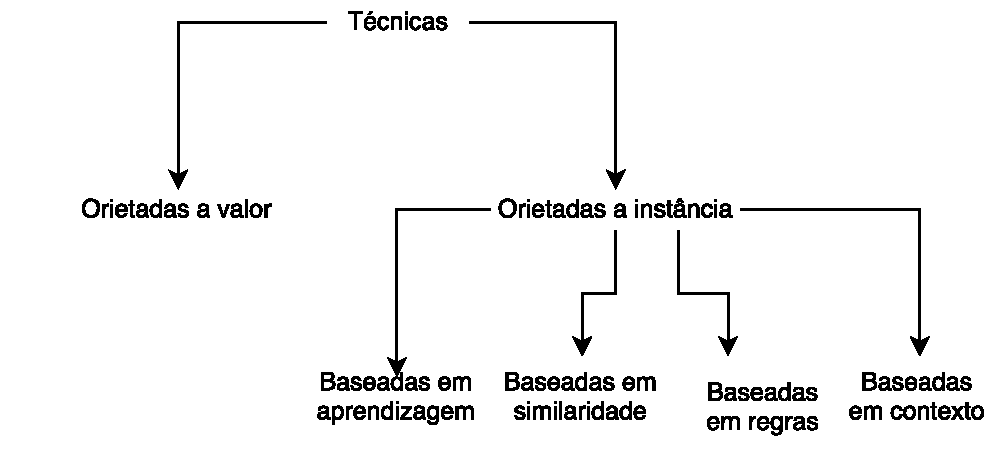
\includegraphics[width=0.85\textwidth]{./imagens/im_techniques.pdf}
	\caption{Técnicas para correspondência de instâncias}
	\footnotesize{Fonte: adaptado de \cite{castano2011ontology}.}
	\label{fig:im_techniques}
\end{figure}

Na segunda categoria, estão concentradas as técnicas orientadas à instância. 

\textbf{Baseada em aprendizagem:} Utiliza grupos de treinamento bem como técnicas de aprendizagem de máquina, como Máquina de Vetor de Suporte (\textit{support vector machine}), para definir se os recursos representam a mesma entidade do mundo real.

\textbf{Baseada em similaridade:} Essa técnica enxerga os recursos como um conjunto de valores. Pode utilizar as mesmas funções para comparação entre textos, como a similaridade média para comparar dois recursos. 

\textbf{Baseadas em regras:} Diferente das outras técnicas, esta usa valores booleanos no lugar de valores numéricos. Além disso, esta subcategoria apresenta bons resultados, porém esta abordagem é dependente do domínio. 

\textbf{Baseadas em contexto:} O contexto de um recurso pode ser entendido como os relacionamentos dele com outros recursos. Dessa forma, essa abordagem analisa as instâncias e suas relações.

Conforme as técnicas apresentadas, tem-se que o calculo da similaridade entre recursos é elemento comum entre as aplicações de correspondência de instância.

Para identificar e conectar recursos na Web, a comunidade vem apresentando um número crescente de soluções (ver Figura \ref{fig:oaei_imtools}).a \textit{Ontology Alignment Evaluation Initiative} (OAEI) realiza uma avaliação anual, que consiste em alinhar dois conjuntos de dados pré-definidos e comparar o alinhamento gerado pela solução com o alinhamento de referência. A partir da comparação entre os dois conjuntos de alinhamento, as métricas de precisão, revocação e medida-f são geradas.


\begin{figure}[!h]
        \centering
        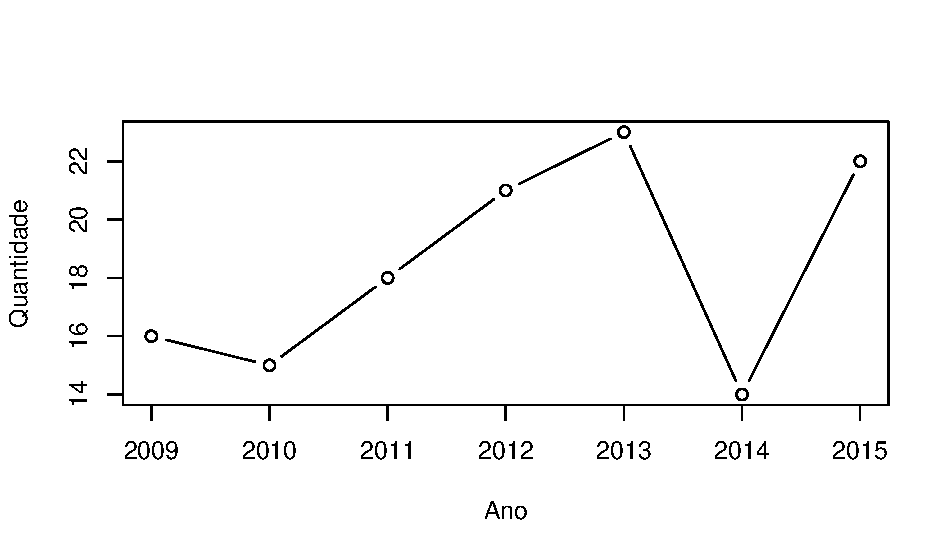
\includegraphics[width=0.9\textwidth]{./imagens/im_tools.pdf}
    \caption{Quantidade de soluções submetidas ao OAEI}
        \footnotesize{Fonte: \cite{cheatham2015results}.}
        \label{fig:oaei_imtools}
\end{figure}

Porém, de acordo com \citeonline{homoceanu2014putting}, apesar dos bons resultados apresentados, as soluções não estão prontas para alinhar dados automaticamente de forma confiável. Para se chegar a esta conclusão, os autores realizaram um experimento equivalente ao executado pela OAEI, mas utilizando dados reais, que foram obtidos de 5 fontes diferentes (Freebase\footnote{\url{http://www.freebase.com/}}, DBPedia\footnote{\url{http://dbpedia.org}}, LinkedMDB\footnote{\url{http://www.linkedmdb.org}}, DrugBase\footnote{\url{http://www.drugbase.de/de/}} e NewYork Times\footnote{\url{http://www.nytimes.com}}), que podem ser obtidos através do endereço \url{http://www.ifis.cs.tu-bs.de/node/2906}.

No experimento realizado por \citeonline{homoceanu2014putting} foi utilizada uma abordagem de caixa preta, onde qualquer sistema independente de domínio pode ser utilizado na avaliação. Nesse contexto, o SLINT+ \cite{nguyen2012interlinking} foi utilizado por ser uma ferramenta independente de domínio e que não precisa de treinamento. A ferramenta foi avaliada em duas perspectivas. Na primeira perspectiva a transitividade da propriedade \textit{owl:sameAs} foi desconsiderada. Diferentemente da segunda, que considerou a transitividade das correspondências criadas. A Tabela \ref{tab:homoceanu2014putting} apresenta os resultados obtidos no experimento \cite{homoceanu2014putting}.

\begin{table}[h]
	\centering
	\caption{Quantidade de links owl:sameAs, quantidade de links owl:sameAs entre tipos diferentes,precisão. Nas perspectivas sem e com transividade}
	\label{tab:homoceanu2014putting}
	\begin{tabular}{@{}l|lll|lll@{}}
		\toprule
		\multicolumn{1}{c|}{\multirow{2}{*}{$\theta$}} & \multicolumn{3}{c|}{SLINT+}                                                                      & \multicolumn{3}{c}{$cl_{TR}$}                                                                  \\
		\multicolumn{1}{c|}{}                        & \multicolumn{1}{c}{\#sameAs} & \multicolumn{1}{c}{Inter-domínio} & \multicolumn{1}{c|}{Precisão} & \multicolumn{1}{c}{\#sameAs} & \multicolumn{1}{c}{Inter-domínio} & \multicolumn{1}{c}{Precisão} \\ \midrule
		0.95                                         & 8,020                        & 33                                & 0.91                          & 2,055                        & 89                                & 0.20                         \\
		0.75                                         & 16,739                       & 119                               & 0.71                          & 5,498                        & 216                               & 0.15                         \\
		0.50                                         & 17,436                       & 230                               & 0.76                          & 7,038                        & 396                               & 0.09                         \\
		0.25                                         & 25,113                       & 1,734                             & 0.67                          & 14,879                       & 2,408                             & 0.02                         \\ \bottomrule
	\end{tabular}
\end{table}



%Além disso, o experimento permitiu notar que as características do modelo não eram considerados durante o processo de correspondência de instâncias.

Segundo \cite{homoceanu2014putting} e \cite{ferrara2008towards}, uma solução de correspondência de instâncias deveria explorar a modelagem ontológica, que utiliza vocabulários e ontologias para seu desenvolvimento. Essa recomendação se deve ao fato de RDF apenas dá estrutura aos dados, sendo responsabilidade das ontologias dar significado aos conceitos representados. Um modelo ontológico é composto por classes e propriedades, que são descritas através de uma linguagem de descrição de ontologias (e.g. OWL). As classes são utilizadas para representar os conceitos que pertencem ao domínio de interesse, já as propriedades são utilizadas para relacionar conceitos, sendo chamadas de propriedades de objeto (\textit{object properties}) ou relacionar conceitos e dados, sendo chamadas de propriedade de dados (\textit{data properties}). Essas propriedades possuem características como transitividade, simetria e reflexibilidade. Dessa forma, o baixo suporte às características das propriedades pode afetar diretamente na qualidade de soluções de correspondência de instâncias. 
        
Dentre as propriedades com suporte inadequado,  destaca-se a propriedade owl:sameAs, que é responsável por identificar recursos equivalentes. Além disso, essa se trata de uma propriedade transitiva, de forma que se existem dois recursos equivalentes R1 e R2 e existe um terceiro recurso R3 que é equivalente a R2, então R1 é equivalente a R3 como representado na Figura \ref{sameAsSample}. Tais características fazem com que a propriedade owl:sameAs seja uma das  mais utilizadas para alinhar dados na Web. Dessa forma, utilizar ferramentas que levem em consideração as características das propriedades é de grande importância para alinhar dados de forma confiável.


\begin{figure}[h]
	\centering
	\subfloat[owl:sameAs]
	{
		\begin{tikzpicture}[node distance=1cm, auto,]
		%nodes
		\node[ellipse,draw] (r3) {R3};
		
		\node[above=of r3] (dummy) {};
		\node[right= of dummy,ellipse,draw](r2) {R2}
		edge[pil,<->, bend left=45] node[auto] {owl:sameAs} (r3);
		
		\node[left= of dummy,ellipse,draw] (r1) {R1}
		edge[dashed,<->, bend right=45] node[auto] {owl:sameAs} (r3)
		edge[pil,<->, bend left=45] node[auto] {owl:sameAs} (r2);
		\end{tikzpicture}
	}
	\subfloat[Exemplo]
	{
		\begin{tikzpicture}[node distance=1cm, auto,]
		%nodes
		\node[ellipse,draw] (r3) {lattes:perfil\_1};
		
		\node[above=of r3] (dummy) {};
		\node[right= of dummy,ellipse,draw](r2) {dblp:perfil\_2}
		edge[pil,<->, bend left=45] node[auto] {owl:sameAs} (r3);
		
		\node[left= of dummy,ellipse,draw] (r1) {schoolar:perfil\_3}
		edge[dashed,<->, bend right] node[auto] {owl:sameAs} (r3)
		edge[pil,<->, bend left] node[auto] {owl:sameAs} (r2);
		\end{tikzpicture}
		}
		\caption{Transitividade da propriedade owl:sameAs}
		\label{sameAsSample}
\end{figure}


Neste contexto, este trabalho propõe uma abordagem independente de contexto para o alinhamento de dados conectados por meio de um processo de alinhamento que leva em consideração aspectos dos dados e  características do modelo ontológico.
Assim, os recursos/instâncias analisados, além de alinhados através das propriedades de dados, podem ser alinhados através seus relacionamentos. Para isso, propõe-se uma abordagem de alinhamento em cascata. Ademais, a proposta trata o problema do alinhamento entre \textit{datasets} reais, permitindo que seja possível alinhar \textit{datasets} distribuídos na Web de forma confiável.

\section{Problemática e justificativa}
Em um cenário favorável, a tarefa de encontrar recursos correspondentes entre \textit{datasets} pode ser realizada com facilidade. Por outro lado, o mesmo não pode ser dito quando há milhares de instâncias, visto que os recursos necessários para manter uma análise manual tornam esta prática inviável. Além disso, devido ao esforço necessário juntamente com a quantidade de instâncias que devem ser comparadas, tem-se que a qualidade da análise pode ser comprometida.

Sabendo que aumentar a quantidade de recursos não é uma solução, nos deparamos com nosso problema geral:

\textbf{(Problema Geral)} Como simplificar a identificação de instâncias que dizem respeito à mesma entidade do mundo real?

Para manter a qualidade das análises, mesmo com o crescimento dos \textit{datasets}, diversas comunidades utilizam a tecnologia para auxiliar na correspondência de recursos. Dentre essas comunidades, destaca-se a de Banco de Dados (BD), que estuda abordagens para identificar recursos entre bancos de dados diferentes. No entando, \citeonline{araujo2011serimi} ressaltam que apesar das abordagens utilizadas pela comunidade de BD (\textit{Record Linkage}) compartilhar características com as abordagens utilizadas pela comunidade de Dados Conectados (\textit{Instance Matching}), ambas diferenciam-se em alguns aspectos, tais como: semântica dos relacionamentos e flexibilidade do modelo RDF.

Para suportar os aspectos que diferenciam \textit{Record Linkage} de \textit{Instance Matching}, a comunidade de Dados Conectados vêm desenvolvendo abordagens próprias. Essas abordagens vêm se mostrando promissoras diante das avaliações às quais são submetidas. Porém, apesar do desempenho apresentado, diversas soluções deixam a desejar no suporte a aspectos relacionados à semântica do modelo ontológico, comprometendo a qualidade das correspondências geradas.

O que leva ao nosso problema específico.

\textbf{(Problema Específico)} Como melhorar a eficácia das ferramentas para correspondência de instâncias?

Para tanto, é apresentado como questão de pesquisa (\textbf{Q1}) o seguinte questionamento:

\textbf{Q1:} Como se comportam as ferramentas para correspondência de instâncias com relação a eficácia?

\section{Objetivo}


Essa abordagem visa disponibilizar um mecanismo útil que permita alinhar semiautomaticamente recursos entre \textit{datasets} diferentes. Além disso, a proposta também pretende facilitar a identificação e alinhamento de recursos dentro do mesmo \textit{dataset}. 

Apesar de ser um trabalho com enfoque em engenharia de software, as suas contribuições estão mais voltadas para a área de Dados Conectados. Segue algumas dessas contribuições:

\begin{itemize}
        \item Construção de um processo para a correspondência de instâncias que seja independente de contexto;
        \item Implementação de uma abordagem em cascata para a correspondência de instância a partir de instâncias relacionadas;
\end{itemize}


\section{Contribuição e relevância do trabalho}
\label{contribuicao}
Anualmente a OAEI realiza a avaliação de ferramentas para a correspondência de instâncias. Essa avaliação utiliza \textit{datasets} previamente disponibilizados juntamente com uma referência de correspondências entre as instâncias. Essa prática permite que o experimento seja reproduzido, permitindo que os resultados fornecidos pela OAEI sejam validados. Por outro lado, permite também que dos desenvolvedores implementem algoritmos que utilizam computação específica para o \textit{dataset}. Desta forma, é necessário o estudo de abordagens independentes de contexto que sejam capazes de alinhar dados de forma confiável. Além disso, as soluções fornecidas requerem que os \textit{datasets} sejam fornecidos em formato de arquivo, sendo necessário gerar os arquivos dos \textit{datasets} sempre que é necessário realizar a correspondência de instâncias.

Nesse contexto, a proposta apresenta as seguintes contribuições:
\begin{itemize}
\item Desenvolvimento de processo independente de contexto para o alinhamento de dados conectados;
\item Viabilização da execução do alinhamento diretamente dentro do armazenamento de triplas;% * 
\item  Criação de experimento e estudo de caso para avaliar a eficácia das soluções de alinhamento no estado da arte.
\end{itemize}

\section{Estrutura do trabalho}

Esta dissertação está dividida em 7 capítulos. O Capítulo \ref{cap:introducao} introduz a problemática e os objetivos do trabalho proposto, enaltecendo a necessidade de uma abordagem capaz de alinhar dados conectados. No Capítulo \ref{cap:fundamentacao}, são apresentados os conceitos: RDF, Ontologias, Dados Conectados, Algoritmos de similaridade e Alinhamento de Dados Conectados. Além disso, também é apresentado os trabalhos relacionados. Na conclusão do capítulo é apresentada uma tabela comparativa entre a abordagem proposta e os trabalhos relacionados apresentados.

O Capítulo \ref{cap:processo} descreve em detalhes o processo de correspondência de instâncias proposto. O processo foi descrito por intermédio de um diagrama de atividades. A subseção \ref{sub:cascata} descreve em detalhes como é realizado o alinhamento/correspondência em cascata, que é umas das principais contribuições deste trabalho.

O Capítulo \ref{cap:componentes} mostra como a proposta foi desenvolvida, através de um diagrama de componentes. Neste capítulo, todas as etapas do processo bem como os componentes da arquitetura são descritos detalhadamente.

No Capítulo \ref{cap:estudo} é apresentado um estudo de caso. Nele é descrito o QIE, um sistema que apresenta o cruzamento dados da Revista Brasileira de Informática na Educação (RBIE), Simpósio Brasileiro de Informática na Educação (SBIE) e Workshop de informática na Escola (WIE) com dados extraídos da plataforma LATTES. Além disso, é descrito como o processo foi utilizado para alinhar os dados dos pesquisadores e de suas produções científicas entre essas bases.

No Capítulo \ref{cap:experimento}, um experimento foi projetado para avaliar, em termos de eficácia através das métricas de precisão, revocação e medida-f, a abordagem proposta, em comparação com AgreementMakerLite (AML) \cite{fariaoaei} e RiMOM-2016 \cite{zhang2016rimom}. Cada conjunto de alinhamento gerado é avaliado e uma discussão geral é apresentada ao final do capítulo.

Por fim, no Capítulo \ref{cap:conclusao}, são apresentadas as considerações finais deste trabalho. bem como são definidos alguns trabalhos futuros.
